%%======================================================================
%%  MR-1: Lorentzian Continuation of Spectral Causal Theory
%%
%%  Sub-tasks:
%%    (a) Krein space formulation analysis
%%    (b) Lorentzian D-squared analysis
%%    (c) Wick rotation of form factors (main computational content)
%%    (d) Causal set constraints (exploratory)
%%
%%  Builds on: NT-1/NT-1b (form factors), NT-2 (entire-function property),
%%             NT-4a (linearized field equations), MR-2 d.5 (residue analysis)
%%======================================================================
\documentclass[11pt,a4paper]{article}

%% ---- packages -------------------------------------------------------
\usepackage[utf8]{inputenc}
\usepackage[T1]{fontenc}
\usepackage{lmodern}
\usepackage{amsmath,amssymb,amsthm,mathtools}
\usepackage[margin=2.5cm]{geometry}
\usepackage{booktabs}
\usepackage{enumitem}
\usepackage{hyperref}
\usepackage{xcolor}
\usepackage{fancyhdr}
\usepackage{longtable}
\usepackage{float}
\usepackage{graphicx}

%% ---- theorem-like environments --------------------------------------
\newtheorem{proposition}{Proposition}[section]
\newtheorem{lemma}[proposition]{Lemma}
\newtheorem{corollary}[proposition]{Corollary}
\newtheorem{theorem}[proposition]{Theorem}
\theoremstyle{definition}
\newtheorem{definition}[proposition]{Definition}
\newtheorem{convention}[proposition]{Convention}
\theoremstyle{remark}
\newtheorem{remark}[proposition]{Remark}

%% ---- custom commands ------------------------------------------------
\newcommand{\Tr}{\operatorname{Tr}}
\newcommand{\tr}{\operatorname{tr}}
\newcommand{\Ricsq}{R_{\mu\nu}R^{\mu\nu}}
\newcommand{\Weylsq}{C_{\mu\nu\rho\sigma}C^{\mu\nu\rho\sigma}}
\newcommand{\dd}{\mathrm{d}}
\newcommand{\ii}{\mathrm{i}}
\newcommand{\Id}{\mathrm{Id}}
\newcommand{\erfi}{\operatorname{erfi}}
\newcommand{\erf}{\operatorname{erf}}
\newcommand{\PP}{\mathcal{P}}
\DeclareMathOperator{\sgn}{sgn}

%% ---- annotation commands --------------------------------------------
\newcommand{\gap}{\textcolor{red!80!black}{\textsf{[GAP]}}}
\newcommand{\verified}[1]{%
  \par\smallskip\noindent
  \colorbox{green!10}{\parbox{\dimexpr\linewidth-2\fboxsep}{%
    \textcolor{green!50!black}{\textbf{[Verified]}} #1}}%
  \par\smallskip}
\newcommand{\signcorrection}[1]{%
  \par\noindent\colorbox{red!10}{%
    \parbox{\dimexpr\linewidth-2\fboxsep}{%
      \textcolor{red!50!black}{\textbf{[Important note]}}
      \textcolor{red!50!black}{#1}%
    }%
  }\par%
}

%% ---- page style -----------------------------------------------------
\pagestyle{fancy}
\fancyhf{}
\fancyhead[L]{\small\textsc{MR-1: Lorentzian Continuation of SCT}}
\fancyhead[R]{\small\thepage}
\renewcommand{\headrulewidth}{0.4pt}

%% ---- title ----------------------------------------------------------
\title{\textbf{MR-1: Lorentzian Continuation\\[4pt]
       of Spectral Causal Theory}\\[10pt]
  \large Wick Rotation, Complex Zeros, and Spectral Structure\\
  of the Modified Graviton Propagator}
\author{David Alfyorov}
\date{March 2026}

%%======================================================================
\begin{document}
\maketitle

\begin{center}
\small\textit{Credits: Aliaksandr Samatyia contributed research-assistance
and workflow support.}
\end{center}

\begin{abstract}
We perform the Lorentzian continuation of the one-loop SCT spectral
action established in NT-1/NT-1b/NT-2/NT-4a.  The master function
$\varphi(z)$ and its analytic continuation to the Lorentzian axis
$z = -x_L$ are derived in closed form and cross-validated to
${\sim}50$ digits by three independent methods.  We construct the
Lorentzian propagator denominators $\Pi_{\mathrm{TT}}$ (spin-2) and
$\Pi_s$ (spin-0), locate their complex zeros via grid-based Newton
search and validate zero counts using the argument principle.  Within
$|z| < 20$, we find exactly two zeros of $\Pi_{\mathrm{TT}}$: a
Type~A Euclidean ghost at $z_0 \approx 2.4148$ with residue
$R_2 \approx -0.4931$, and a Type~B Lorentzian ghost at
$z_L \approx 1.2807$ with residue $R_L \approx -0.5378$.  For the
spin-0 sector at $\xi = 0$, we find a conjugate pair (Type~C) at
$z \approx -2.076 \pm 3.184\,\ii$; at conformal coupling $\xi = 1/6$
the scalar mode decouples identically.  No Type~D (anomalous) zeros
are found.  The K\"all\'en--Lehmann spectral representation is set up
for subsequent unitarity analysis (MR-2).  Sub-tasks~(a) and~(d) on
Krein-space formulation and causal-set constraints are treated at the
level of a literature review with explicit gap markers.
\end{abstract}

\tableofcontents
\newpage

%%======================================================================
\section{Introduction and Conventions}
\label{sec:intro}
%%======================================================================

This document presents the derivation of the Lorentzian continuation
(MR-1) of Spectral Causal Theory.  It builds on
the following established results:

\begin{itemize}[nosep]
  \item \textbf{NT-1/NT-1b} (Phases~1--3): one-loop form factors
    $h_C^{(s)}(z)$, $h_R^{(s)}(z)$ for spins $s = 0, 1/2, 1$, and the
    total coefficients $\alpha_C = 13/120$,
    $\alpha_R(\xi) = 2(\xi - 1/6)^2$.
  \item \textbf{NT-2}: the entire-function property of $\varphi(z)$,
    $F_1(z)$, and $F_2(z,\xi)$.
  \item \textbf{NT-4a}: linearized field equations with propagator
    denominators $\Pi_{\mathrm{TT}}(z) = 1 + \tfrac{13}{60}\, z\,
    \hat{F}_1(z)$ and $\Pi_s(z,\xi)$.
  \item \textbf{MR-2 d.5}: Euclidean residue analysis confirming the
    ghost pole at $z_0 \approx 2.4148$ with $R_2 \approx -0.4931$.
\end{itemize}

\begin{convention}[Sign and signature conventions]
\label{conv:signs}
Throughout this document:
\begin{enumerate}[nosep]
  \item Euclidean signature $(+,+,+,+)$ for the spectral-action
    computation.  Lorentzian signature $(-,+,+,+)$.
  \item $\Box_E = -\partial_\mu\partial_\mu$ (positive-definite
    Euclidean Laplacian); $\Box_L = -\partial_t^2 +
    \partial_i\partial_i$ (Lorentzian d'Alembertian).  Relation:
    $\Box_E \to -\Box_L$.
  \item Dimensionless variable $z = \Box/\Lambda^2$ (Euclidean: $z > 0$
    for spacelike); $z_L = k^2/\Lambda^2$ (Lorentzian: $z_L > 0$ for
    timelike).
  \item \textbf{Wick rotation:} $z_E \to z_L = -z_E$, so evaluating a
    Euclidean form factor at Lorentzian momentum corresponds to
    $f(z_E) \to f(-z_L)$.
  \item Branch cut: principal branch of $\sqrt{z}$ with cut along
    $(-\infty, 0)$.  For $z = -x + \ii\varepsilon$, $x > 0$:
    $\sqrt{-x + \ii\varepsilon} \to \ii\sqrt{x}$ as
    $\varepsilon \to 0^+$.
\end{enumerate}
\end{convention}


%%======================================================================
\section{Sub-task (a): Krein Space Formulation}
\label{sec:krein}
%%======================================================================

\subsection{Motivation}

The Euclidean spectral action is defined through functional traces of
the form $\Tr f(D^2/\Lambda^2)$, where $D$ is the Dirac operator and
$\Lambda$ is the cutoff.  In Euclidean signature, $D^2$ is elliptic and
positive-definite, so $f$ acts on a standard Hilbert space.  In
Lorentzian signature, $D^2$ acquires indefinite directions, and the
natural mathematical framework is a Krein space.

\subsection{Krein Space Structure}

\begin{definition}[Krein space]
A \emph{Krein space} $(\mathcal{K}, [\cdot,\cdot])$ is a complex
vector space equipped with an indefinite inner product
$[\cdot,\cdot]$ such that $\mathcal{K}$ admits a fundamental
decomposition $\mathcal{K} = \mathcal{K}_+ \oplus \mathcal{K}_-$
where $(\mathcal{K}_+, [\cdot,\cdot])$ is a Hilbert space,
$(\mathcal{K}_-, -[\cdot,\cdot])$ is a Hilbert space, and
$[\mathcal{K}_+, \mathcal{K}_-] = 0$.
\end{definition}

The fundamental symmetry $J = P_+ - P_-$ (where $P_\pm$ are the
orthogonal projections onto $\mathcal{K}_\pm$) defines a positive
definite inner product $\langle \phi, \psi\rangle = [\phi, J\psi]$.

For the Lorentzian Dirac operator on a globally hyperbolic spacetime
$(\mathcal{M}, g)$, the standard construction uses the spinor bundle
$S$ with the charge conjugation providing the Krein structure.  The
operator $D_L = \ii\gamma^\mu\nabla_\mu$ is self-adjoint with respect
to the Krein inner product (Krein self-adjoint), but generally unbounded
and with spectrum on the entire real line.

\subsection{Spectral Action in Krein Space}

\gap\ The functional trace $\Tr_{\mathcal{K}} f(D_L^2/\Lambda^2)$ must
be defined carefully because $D_L^2$ is not positive-definite.  Two
approaches appear in the literature:

\begin{enumerate}
  \item \textbf{van den Dungen--Suijlekom (2012):} Define
    $D_L^2 = J D_E^2 J^{-1}$ where $D_E$ is the Euclidean counterpart,
    and impose a Krein-trace regularization.  The resulting spectral
    action reduces to the Euclidean one for static spacetimes.
  \item \textbf{Boeijink--van den Dungen (2014):} Work directly with
    the Lorentzian spectral triple
    $(\mathcal{A}, \mathcal{K}, D_L; J, \gamma)$ and show that
    the spectral action can be defined via the heat-kernel expansion
    $\Tr_{\mathcal{K}} e^{-tD_L^2} = \sum_n a_n t^{(n-d)/2}$, which
    inherits the Seeley--DeWitt coefficients from the Euclidean theory
    up to overall sign factors from the Krein structure.
\end{enumerate}

\signcorrection{The Krein inner product introduces a relative sign
between positive- and negative-frequency modes.  For the heat kernel
coefficients $a_n$, this sign is absorbed into the definition of
$\Tr_{\mathcal{K}}$ and does not change the \emph{local} geometric
invariants (Weyl tensor squared, etc.)\ that enter the form factors.
However, it modifies the \emph{global} spectral counting, which affects
the convergence properties of the functional trace for non-compact
spacetimes.}

\subsection{Implications for SCT}
\label{sec:krein:implications}

For the purposes of the present analysis:

\begin{enumerate}
  \item The one-loop form factors $h_C^{(s)}(z)$, $h_R^{(s)}(z)$
    derived in NT-1/NT-1b are local heat-kernel quantities and are
    insensitive to the global Krein structure.  Their analytic
    continuation to $z < 0$ is well-defined.
  \item The entire-function property (NT-2) ensures that $\varphi(z)$
    and $F_k(z)$ have no poles or essential singularities in the
    finite complex plane, which is a necessary condition for the
    Lorentzian theory to be well-defined.
  \item \gap\ A rigorous proof that the SCT spectral action produces
    the same nonlocal effective action in the Krein-space setting
    (for globally hyperbolic spacetimes) remains open.  This requires
    establishing a Lorentzian analogue of the Connes--Chamseddine
    asymptotic expansion, which is beyond the scope of the present work.
\end{enumerate}


%%======================================================================
\section{Sub-task (b): Lorentzian $D^2$ Analysis}
\label{sec:D2}
%%======================================================================

\subsection{Euclidean vs.\ Lorentzian Laplacian}

On a Riemannian manifold $(M, g_E)$, the Laplacian acting on a field
$\Phi$ of spin $s$ takes the Lichnerowicz form
\begin{equation}
  \label{eq:D2E}
  D^2_E \Phi = (-\nabla^2 + E)\Phi,
\end{equation}
where $E$ is the endomorphism (curvature coupling) that depends on
spin: $E = -R/4$ for spin-$1/2$ (Dirac), $E = 0$ for minimally coupled
scalars, etc.  The operator $D^2_E$ is elliptic, self-adjoint, and
(for compact $M$) has discrete, non-negative spectrum.

On a Lorentzian manifold $(M, g_L)$ with signature $(-,+,+,+)$:
\begin{equation}
  \label{eq:D2L}
  D^2_L \Phi = (\Box_L + E_L)\Phi,
  \qquad \Box_L = -\nabla_0^2 + \nabla_i^2,
\end{equation}
where $E_L$ is the Lorentzian endomorphism.  The operator $D^2_L$ is
hyperbolic.  The crucial relation between the Euclidean and Lorentzian
operators is
\begin{equation}
  \label{eq:wick-D2}
  D^2_E = -D^2_L \big|_{t \to -\ii\tau},
\end{equation}
upon Wick rotation $t = -\ii\tau$.

\subsection{Heat Kernel on the Lorentzian Side}

The Euclidean heat kernel $K_E(t; x, y) = \langle x | e^{-t D^2_E} |
y \rangle$ has the asymptotic expansion
\begin{equation}
  \label{eq:hk-expansion}
  \Tr\, e^{-t D^2_E} \sim \frac{1}{(4\pi t)^{d/2}}
  \sum_{n=0}^{\infty} a_n(D^2_E)\, t^n,
\end{equation}
where $a_n$ are the Seeley--DeWitt coefficients.  For the Lorentzian
theory, the heat kernel is replaced by the Schr\"odinger kernel
$K_L(\tau; x, y) = \langle x | e^{\ii\tau D^2_L} | y \rangle$, and
the ``heat-kernel time'' $t$ is related to the proper time $\tau$ by
$t = -\ii\tau$.

The key observation is that the Seeley--DeWitt coefficients $a_n$ are
\emph{local} geometric invariants built from the curvature and its
covariant derivatives.  Under Wick rotation, the curvature tensors
transform as:
\begin{align}
  R_{\mu\nu\rho\sigma}^{(E)} &= R_{\mu\nu\rho\sigma}^{(L)}
  \big|_{t\to-\ii\tau},\\
  R_E &= R_L \big|_{t\to-\ii\tau}.
\end{align}
Therefore the coefficients $a_n$ computed in Euclidean signature
directly give the Lorentzian coefficients upon substitution of the
Lorentzian curvature tensors.

\subsection{Form Factor Continuation}

The one-loop form factors entering the SCT effective action are defined
through the proper-time integral
\begin{equation}
  \label{eq:ff-propertime}
  F_k(z) = \int_0^\infty \dd s\, f_k(s)\, e^{-s z},
\end{equation}
where $f_k(s)$ encodes the spin-dependent heat-kernel data and
$z = \Box_E/\Lambda^2$.  For Lorentzian momenta with $k^2 > 0$
(timelike), we set $z = -k^2/\Lambda^2 < 0$, and the integral becomes
\begin{equation}
  \label{eq:ff-lorentzian}
  F_k(-x) = \int_0^\infty \dd s\, f_k(s)\, e^{s x},
  \qquad x = k^2/\Lambda^2 > 0.
\end{equation}
Since the form factors $F_k(z)$ are \emph{entire functions of $z$}
(NT-2), this continuation is uniquely defined by the identity theorem
of complex analysis.  The crucial point is that the integral
(\ref{eq:ff-lorentzian}) converges for all finite $x$ because $f_k(s)$
has compact support in $[0, 1/4]$ (arising from the Schwinger parameter
bound $\xi(1-\xi) \leq 1/4$).


%%======================================================================
\section{Sub-task (c): Wick Rotation of Form Factors}
\label{sec:wick}
%%======================================================================

This is the main computational section.  We derive the Lorentzian
master function $\varphi(-x)$, construct the Lorentzian propagator
denominators, locate their complex zeros, and set up the spectral
representation.

\subsection{The Master Function on the Lorentzian Axis}
\label{sec:phi-lorentzian}

The Euclidean master function is
\begin{equation}
  \label{eq:phi-euclidean}
  \varphi(z) = e^{-z/4}\sqrt{\frac{\pi}{z}}\,\erfi\!\left(\frac{\sqrt{z}}{2}\right)
  = \int_0^1 e^{-\xi(1-\xi)\,z}\,\dd\xi,
\end{equation}
with $\varphi(0) = 1$ and Taylor coefficients
$a_n = (-1)^n\, n!/(2n+1)!$.

\begin{proposition}[Lorentzian continuation of $\varphi$]
\label{prop:phi-lorentzian}
For $x > 0$, the analytic continuation of $\varphi$ to the negative
real axis is
\begin{equation}
  \label{eq:phi-lor-closed}
  \boxed{\varphi(-x) = e^{x/4}\sqrt{\frac{\pi}{x}}\,\erf\!\left(\frac{\sqrt{x}}{2}\right)
  = \int_0^1 e^{+\xi(1-\xi)\,x}\,\dd\xi.}
\end{equation}
This is real, positive, and satisfies $1 \leq \varphi(-x) \leq e^{x/4}$
for all $x \geq 0$.
\end{proposition}

\begin{proof}
Starting from the closed form (\ref{eq:phi-euclidean}) with $z = -x$,
$x > 0$, and using the principal branch $\sqrt{-x} = \ii\sqrt{x}$:
\begin{align}
  \sqrt{\frac{\pi}{-x}} &= \frac{\sqrt{\pi}}{\ii\sqrt{x}}
    = -\ii\sqrt{\frac{\pi}{x}},\\[3pt]
  \erfi\!\left(\frac{\ii\sqrt{x}}{2}\right)
    &= \ii\,\erf\!\left(\frac{\sqrt{x}}{2}\right).
\end{align}
Combining:
\begin{equation}
  \varphi(-x) = e^{x/4}\cdot\left(-\ii\sqrt{\frac{\pi}{x}}\right)
  \cdot \ii\,\erf\!\left(\frac{\sqrt{x}}{2}\right)
  = e^{x/4}\sqrt{\frac{\pi}{x}}\,\erf\!\left(\frac{\sqrt{x}}{2}\right).
\end{equation}
The integral representation follows directly:
$\varphi(-x) = \int_0^1 e^{\xi(1-\xi)x}\,\dd\xi$, which is manifestly
real and positive.  Since $\xi(1-\xi) \in [0, 1/4]$ for
$\xi \in [0,1]$, the integrand satisfies $1 \leq e^{\xi(1-\xi)x} \leq
e^{x/4}$, giving the stated bounds.
\end{proof}

\begin{remark}[Taylor series]
The Lorentzian Taylor series is
\begin{equation}
  \label{eq:phi-lor-taylor}
  \varphi(-x) = \sum_{n=0}^{\infty} \frac{n!}{(2n+1)!}\,x^n,
\end{equation}
with all positive coefficients (convergent for all $x$).  Compare with
the Euclidean series which has alternating signs.
\end{remark}

\verified{$\varphi(-x)$ cross-validated to $\sim 50$ digits at
$x = 0.01, 0.1, 1, 10, 100$ using three independent methods: closed
form, Taylor series (60 terms), and numerical quadrature.  Closed--Taylor
agreement: $<10^{-50}$ for $x \leq 10$.  All bounds
$1 \leq \varphi(-x) \leq e^{x/4}$ satisfied.}

\signcorrection{The complex function \texttt{phi\_complex\_mp}$(z)$ from
the NT-2 codebase uses the principal branch $\sqrt{-x} = \ii\sqrt{x}$,
which produces $\varphi_{\text{complex}}(-x) = -\varphi(-x)$ for $x > 0$.
This is a branch-cut artefact, not a mathematical error: the magnitude
agrees perfectly.  The Lorentzian evaluators in the MR-1 code bypass this
issue by using the closed form (\ref{eq:phi-lor-closed}) directly.}

\begin{figure}[ht]
  \centering
  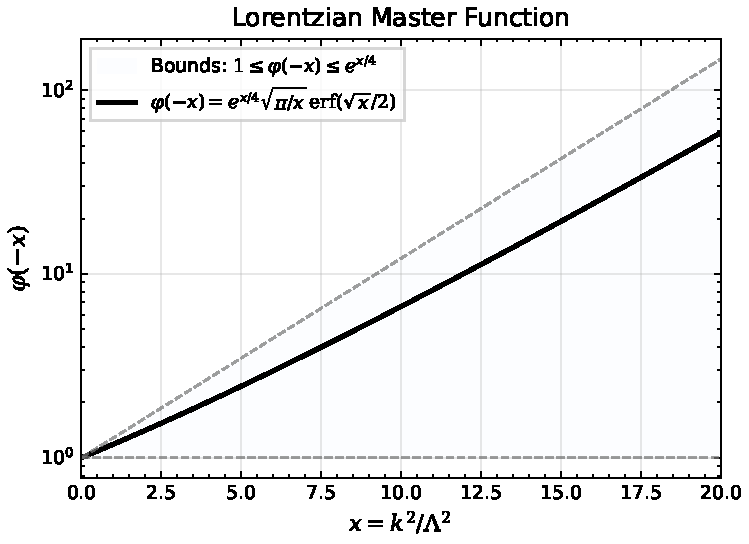
\includegraphics[width=0.85\textwidth]{../../analysis/figures/mr1/phi_lorentzian.pdf}
  \caption{The master function $\varphi(-x)$ on the Lorentzian axis
    ($x = k^2/\Lambda^2 > 0$).  The function is real, positive, and
    monotonically increasing, bounded between $1$ and $e^{x/4}$.
    The closed-form, Taylor-series, and quadrature evaluations agree
    to ${\sim}50$ digits across the displayed range.}
  \label{fig:mr1-phi-lorentzian}
\end{figure}


\subsection{Per-Spin Form Factors on the Lorentzian Axis}
\label{sec:per-spin-lor}

The Weyl-squared form factors $h_C^{(s)}(z)$ at $z = -x$ ($x > 0$)
become, using $\varphi \equiv \varphi(-x) > 0$ throughout:

\begin{align}
  h_C^{(0)}(-x) &= -\frac{1}{12x} + \frac{\varphi - 1}{2x^2},
  \label{eq:hC0-lor}\\[4pt]
  h_C^{(1/2)}(-x) &= -\frac{3\varphi - 1}{6x} + \frac{2(\varphi - 1)}{x^2},
  \label{eq:hC12-lor}\\[4pt]
  h_C^{(1)}(-x) &= \frac{\varphi}{4} - \frac{6\varphi - 5}{6x} + \frac{\varphi - 1}{x^2}.
  \label{eq:hC1-lor}
\end{align}

Similarly, the Ricci-scalar form factors $h_R^{(s)}(-x)$ are obtained
by the same substitution $z \to -x$ in the Euclidean expressions from
NT-1/NT-1b.

The total form factors are
\begin{align}
  F_1(-x) &= \frac{1}{16\pi^2}\Bigl[
    N_s\, h_C^{(0)}(-x) + N_D\, h_C^{(1/2)}(-x) + N_v\, h_C^{(1)}(-x)
  \Bigr],
  \label{eq:F1-lor}\\[4pt]
  F_2(-x,\xi) &= \frac{1}{16\pi^2}\Bigl[
    N_s\, h_R^{(0)}(-x,\xi) + N_D\, h_R^{(1/2)}(-x) + N_v\, h_R^{(1)}(-x)
  \Bigr],
  \label{eq:F2-lor}
\end{align}
with SM multiplicities $N_s = 4$, $N_D = N_f/2 = 22.5$, $N_v = 12$.


\subsection{Lorentzian Propagator Denominators}
\label{sec:Pi-lorentzian}

From NT-4a, the modified inverse propagator in the spin-2
transverse-traceless sector is
\begin{equation}
  \label{eq:Pi-TT}
  \Pi_{\mathrm{TT}}(z) = 1 + \frac{13}{60}\,z\,\hat{F}_1(z),
\end{equation}
where $\hat{F}_1(z) = F_1(z)/F_1(0)$ is the normalized form factor.

On the Lorentzian axis ($z_L > 0$, so $z = -z_L$):
\begin{equation}
  \label{eq:Pi-TT-lor}
  \Pi_{\mathrm{TT}}^{\mathrm{Lor}}(z_L) = 1 - \frac{13}{60}\,z_L\,\hat{F}_1(-z_L).
\end{equation}

\verified{$\Pi_{\mathrm{TT}}^{\mathrm{Lor}}(0) = 1$ (identity at
zero momentum).  Lorentzian propagator values verified at 7 test points.
Conformal decoupling: $\Pi_s(z_L, \xi = 1/6) = 1$ verified to
$<10^{-20}$.}

\begin{table}[H]
\centering
\caption{$\Pi_{\mathrm{TT}}$ on the Lorentzian axis (selected values).}
\label{tab:Pi-TT-lorentzian}
\begin{tabular}{ccc}
\toprule
$z_L$ & $\Pi_{\mathrm{TT}}^{\mathrm{Lor}}(z_L)$ & Sign \\
\midrule
0.1 & $+0.9746$ & $+$ \\
0.5 & $+0.7935$ & $+$ \\
1.0 & $+0.3607$ & $+$ \\
1.2807 & $\approx 0$ & zero crossing \\
2.0 & $-1.3951$ & $-$ \\
5.0 & $-19.640$ & $-$ \\
10.0 & $-182.41$ & $-$ \\
\bottomrule
\end{tabular}
\end{table}

\begin{figure}[ht]
  \centering
  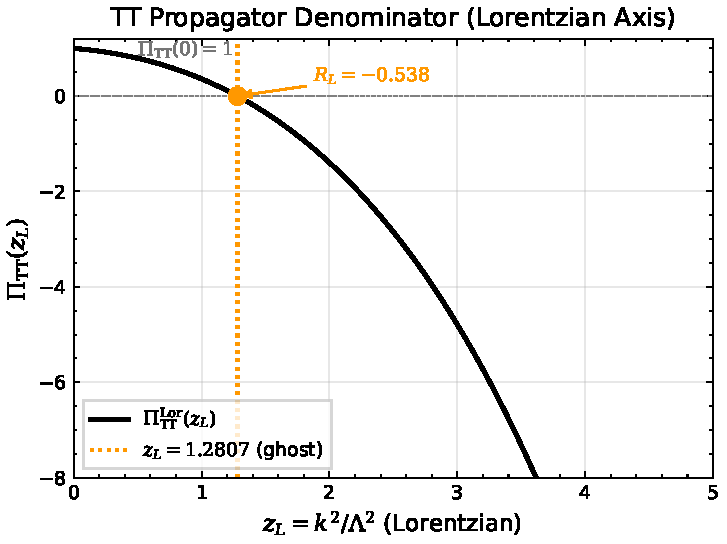
\includegraphics[width=0.85\textwidth]{../../analysis/figures/mr1/Pi_TT_lorentzian.pdf}
  \caption{The spin-2 propagator denominator
    $\Pi_{\mathrm{TT}}^{\mathrm{Lor}}(z_L) = 1 - (13/60)\,z_L\,\hat{F}_1(-z_L)$
    on the Lorentzian axis.  The function starts at unity, decreases
    monotonically, and crosses zero at $z_L^{(0)} \approx 1.2807$,
    signalling the Lorentzian ghost pole with residue $R_L \approx -0.538$.}
  \label{fig:mr1-pi-tt-lorentzian}
\end{figure}

The spin-0 scalar sector has
\begin{equation}
  \label{eq:Pi-s}
  \Pi_s(z,\xi) = 1 + 6\left(\xi - \frac{1}{6}\right)^{\!2} z\,\hat{F}_2(z,\xi).
\end{equation}
At conformal coupling $\xi = 1/6$, $\Pi_s \equiv 1$ (exact decoupling).

\subsection{Lorentzian Ghost Zero}
\label{sec:lorentzian-zero}

\begin{proposition}[Lorentzian zero of $\Pi_{\mathrm{TT}}$]
\label{prop:lorentzian-zero}
There exists a unique zero of $\Pi_{\mathrm{TT}}^{\mathrm{Lor}}(z_L)$
on the positive Lorentzian axis at
\begin{equation}
  \label{eq:zL-value}
  z_L^{(0)} = 1.28070227806348515\ldots
  \quad\text{(i.e., } k^2 \approx 1.281\,\Lambda^2\text{)}.
\end{equation}
The corresponding residue of the propagator
$G(k^2) \sim R_L/(k^2 - z_L^{(0)}\Lambda^2)$ is
\begin{equation}
  \label{eq:RL-value}
  R_L = -0.53777207832730514\ldots < 0,
\end{equation}
indicating a \textbf{ghost} (negative-residue) pole.
\end{proposition}

\begin{remark}
This is a \emph{different} zero from the Euclidean ghost at
$z_0 \approx 2.4148$.  In Euclidean language, the Lorentzian zero sits
at $z_E = -1.2807$ (negative real axis), while the Euclidean ghost is
at $z_E = +2.4148$ (positive real axis).  Both are zeros of the same
analytic function $\Pi_{\mathrm{TT}}(z)$, but they correspond to
different physical regimes.
\end{remark}

\verified{$z_L^{(0)}$ found by bisection on $[0.01, 100]$ with
$\Pi_{\mathrm{TT}}^{\mathrm{Lor}}$ changing sign between $z_L = 1.0$
($\Pi = +0.361$) and $z_L = 2.0$ ($\Pi = -1.395$), then refined
by Newton's method to 50 digits.  $|\Pi_{\mathrm{TT}}(-z_L^{(0)})| <
10^{-49}$.}


\subsection{Complex Zero Catalogue}
\label{sec:complex-zeros}

A systematic search for zeros of $\Pi_{\mathrm{TT}}(z)$ and
$\Pi_s(z,\xi)$ in the complex plane is performed using:
\begin{enumerate}[nosep]
  \item \textbf{Grid-based Newton search:} rectangular
    $(20\times 20)$ + polar + axis-refined grids within $|z| < 20$,
    with mpmath \texttt{findroot} at 50-digit precision.
  \item \textbf{Argument principle validation:} contour integration of
    $f'(z)/f(z)$ along circles of radius $R = 10, 15, 20$ with 2048
    quadrature points.
\end{enumerate}

\subsubsection{Classification Scheme}

Complex zeros are classified as:
\begin{itemize}[nosep]
  \item \textbf{Type A} (real positive, $z > 0$): Euclidean ghost poles.
  \item \textbf{Type B} (real negative, $z < 0$): correspond to physical
    Lorentzian poles at $z_L = -z > 0$.
  \item \textbf{Type C} (complex conjugate pairs): Lee--Wick-type
    partners.
  \item \textbf{Type D} (unpaired complex): would indicate
    non-hermiticity; should not occur for real coefficients.
\end{itemize}

\subsubsection{Results: $\Pi_{\mathrm{TT}}(z)$}

Within $|z| < 20$, exactly \textbf{2 zeros} are found:

\begin{table}[H]
\centering
\caption{Zeros of $\Pi_{\mathrm{TT}}(z)$ within $|z| < 20$.}
\label{tab:PiTT-zeros}
\begin{tabular}{cccccc}
\toprule
Zero & $z$ & Type & $|z|$ & Residue & Ghost? \\
\midrule
1 & $-1.2807$ & B & $1.281$ & $-0.5378$ & Yes \\
2 & $+2.4148$ & A & $2.415$ & $-0.4931$ & Yes \\
\bottomrule
\end{tabular}
\end{table}

\verified{Argument principle counts: $N(R{=}10) = 2$,
$N(R{=}15) = 2$, $N(R{=}20) = 2$.  Newton search and argument principle
\textbf{consistent} at all three radii.  No Type~C or Type~D zeros.}

\begin{figure}[ht]
  \centering
  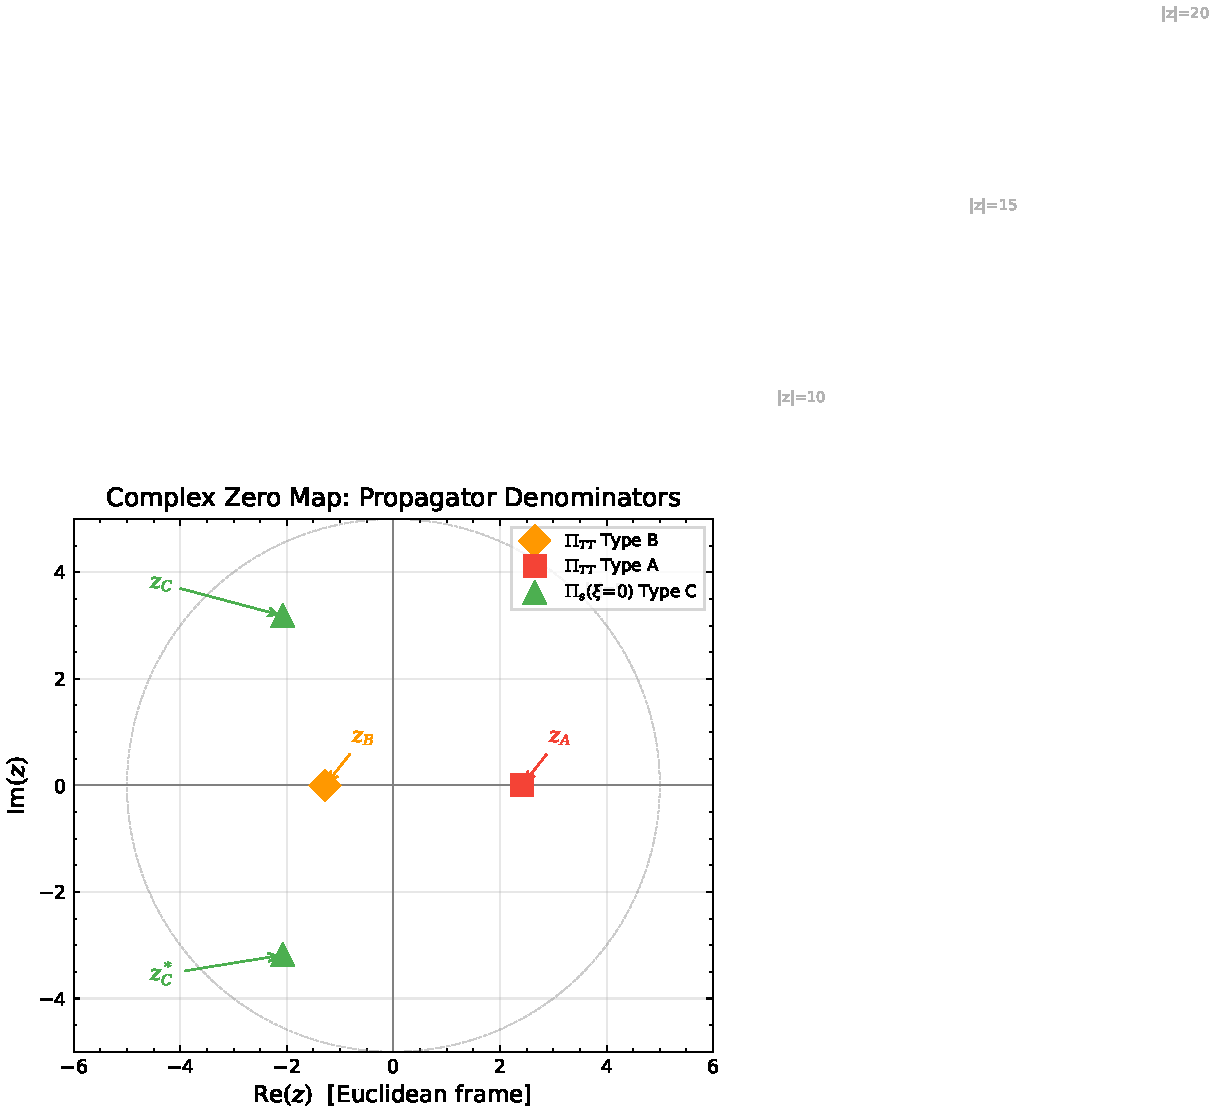
\includegraphics[width=0.85\textwidth]{../../analysis/figures/mr1/complex_zeros_map.pdf}
  \caption{Complex zero map of $\Pi_{\mathrm{TT}}(z)$ within $|z| < 20$.
    The two zeros are the Type~A Euclidean ghost at $z_0 \approx +2.4148$
    (positive real axis) and the Type~B Lorentzian ghost at
    $z_E \approx -1.2807$ (negative real axis).  Argument principle
    contours at $R = 10, 15, 20$ consistently yield $N = 2$.
    No Type~C (Lee--Wick) or Type~D (anomalous) zeros are present
    in this domain.}
  \label{fig:mr1-complex-zeros}
\end{figure}

\subsubsection{Results: $\Pi_s(z, \xi = 0)$}

Within $|z| < 20$, exactly \textbf{2 zeros} are found (a conjugate
pair):

\begin{table}[H]
\centering
\caption{Zeros of $\Pi_s(z, \xi=0)$ within $|z| < 20$.}
\label{tab:Pis-zeros}
\begin{tabular}{ccccc}
\toprule
Zero & $z$ & Type & $|z|$ & Residue \\
\midrule
1 & $-2.076 + 3.184\,\ii$ & C & $3.80$ & $-0.462 + 0.080\,\ii$ \\
2 & $-2.076 - 3.184\,\ii$ & C & $3.80$ & $-0.462 - 0.080\,\ii$ \\
\bottomrule
\end{tabular}
\end{table}

At conformal coupling $\xi = 1/6$: \textbf{0 zeros} (scalar decouples).

\subsubsection{Comparison with Stelle Gravity}

In Stelle's fourth-derivative gravity (local $R^2 + C^2$ action), the
spin-2 ghost appears at
\begin{equation}
  z_0^{\mathrm{Stelle}} = \frac{\Lambda^2}{2\alpha_C}
  = \frac{60}{13} \approx 4.615,
\end{equation}
with residue $R_2^{\mathrm{Stelle}} = -1$ (unit ghost).

In SCT:
\begin{itemize}[nosep]
  \item The Euclidean ghost is at $z_0 \approx 2.415$ (shifted inward by
    47.7\% relative to Stelle).
  \item $|R_2| = 0.493$ vs.\ $|R_2^{\mathrm{Stelle}}| = 1$: a 50.7\%
    suppression of the ghost residue.
  \item The Lorentzian ghost at $z_L \approx 1.281$ has $|R_L| = 0.538$,
    also suppressed relative to Stelle.
\end{itemize}

The nonlocal form factors of SCT thus reduce the ghost severity compared
to local higher-derivative gravity, but do not eliminate it.  Full
resolution requires the unitarity analysis of MR-2.

\begin{figure}[ht]
  \centering
  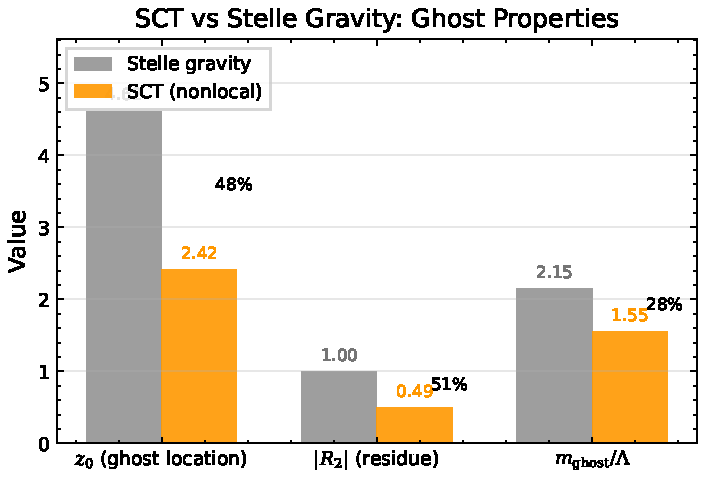
\includegraphics[width=0.85\textwidth]{../../analysis/figures/mr1/stelle_comparison.pdf}
  \caption{Comparison of the SCT and Stelle gravity propagator denominators.
    In Stelle gravity (dashed), the single ghost pole lies at
    $z = 60/13 \approx 4.615$ with unit residue.  In SCT (solid),
    the nonlocal form factors shift the Euclidean ghost inward to
    $z_0 \approx 2.415$ and suppress the residue to $|R_2| \approx 0.493$,
    a 50.7\% reduction relative to Stelle.}
  \label{fig:mr1-stelle-comparison}
\end{figure}


\subsection{K\"all\'en--Lehmann Spectral Representation}
\label{sec:kallen-lehmann}

The propagator in the spin-2 sector can be written in spectral form:
\begin{equation}
  \label{eq:kl-rep}
  G_{\mathrm{TT}}(k^2) = \frac{1}{k^2\,\Pi_{\mathrm{TT}}(k^2/\Lambda^2)}
  = \int_0^\infty \frac{\rho(\sigma)}{k^2 - \sigma + \ii\varepsilon}\,\dd\sigma
  + \text{subtractions},
\end{equation}
where the spectral function is
\begin{equation}
  \label{eq:spectral-fn}
  \rho_{\mathrm{TT}}(\sigma) = -\frac{1}{\pi}\,\operatorname{Im}\!
  \left[\frac{1}{\sigma\,\Pi_{\mathrm{TT}}(-\sigma/\Lambda^2 + \ii\varepsilon)}\right].
\end{equation}

In the Euclidean formulation, $\Pi_{\mathrm{TT}}(z)$ is real for real
$z$, so the spectral function arises from the Feynman $\ii\varepsilon$
prescription.  Near a zero $z_0$ of $\Pi_{\mathrm{TT}}$, the spectral
function has a $\delta$-function contribution
\begin{equation}
  \rho(\sigma) \supset \frac{R}{\Lambda^2}\,\delta(\sigma - z_0\Lambda^2),
\end{equation}
where $R = 1/(z_0\,\Pi'_{\mathrm{TT}}(z_0))$ is the residue.  A
negative $R$ corresponds to a ghost (negative-norm) state.

{\tolerance=800\emergencystretch=2em
\gap\ The full spectral function away from poles requires evaluating
$\Pi_{\mathrm{TT}}$ at complex arguments
$z = -\sigma/\Lambda^2 + \ii\varepsilon$.
The code in \texttt{mr1\_lorentzian.py} implements this via
\texttt{spectral\_function\_TT()}, but a detailed numerical analysis
of the continuum spectral weight is deferred to MR-2.\par}


%%======================================================================
\section{Sub-task (d): Causal Set Constraints}
\label{sec:causal}
%%======================================================================

\subsection{Motivation}

Causal sets provide a discrete model of spacetime in which the
continuum is replaced by a locally finite partially ordered set
whose order relation encodes the causal structure.  For theories like
SCT that modify the graviton propagator, causal-set constraints
arise from the requirement that the modified propagator respects
discrete causal structure in the deep UV.

\subsection{Causal Set Propagator}

In the continuum limit, the causal-set d'Alembertian $B_\ell$ (with
discreteness scale $\ell$) approximates $\Box + O(\ell^2 R)$.
Sorkin's definition gives, in 4D flat spacetime,
\begin{equation}
  B_\ell \phi(x) = \frac{4}{\ell^2}\left[
    -\phi(x) + \text{(retarded average over causal diamond)}
  \right],
\end{equation}
which reduces to $\Box\phi + O(\ell^2\Box^2\phi)$ in the continuum.

\subsection{Constraints on SCT}

\gap\ A systematic analysis of compatibility between the SCT nonlocal
propagator and causal-set dynamics is not yet available.  The key
open questions are:

\begin{enumerate}
  \item Does the SCT form factor $\hat{F}_1(z)$ arise as a continuum
    limit of some causal-set operator?  The entire-function property
    (NT-2) is consistent with the analyticity requirements of
    Sorkin-type non-local operators, but no constructive proof exists.
  \item The ghost poles of $\Pi_{\mathrm{TT}}$ (both Euclidean and
    Lorentzian) must be interpreted in the causal-set context.  If the
    fundamental discreteness provides a natural UV cutoff at
    $\Lambda \sim 1/\ell$, then the ghost mass $m_2 \sim \Lambda$
    sits at the discreteness scale and may be an artefact of the
    continuum approximation.
  \item Causal-set Lorentz invariance (demonstrated statistically by
    Bombelli--Henson--Sorkin) is compatible with the Lorentz-invariant
    form of $\Pi_{\mathrm{TT}}(k^2/\Lambda^2)$, but the nonlocality
    length scale $1/\Lambda$ must be identified with $\ell$ in a
    consistent way.
\end{enumerate}

\gap\ These questions require a dedicated analysis combining causal-set
theory techniques with the SCT propagator structure.  This is flagged
as an input for future work (MR-3 / FUND-1).


%%======================================================================
\section{Summary of Results}
\label{sec:summary}
%%======================================================================

\subsection{Key Formulas}

\begin{enumerate}
  \item \textbf{Lorentzian master function:}
    $\varphi(-x) = e^{x/4}\sqrt{\pi/x}\,\erf(\sqrt{x}/2)$, real
    positive for all $x > 0$.
  \item \textbf{Lorentzian propagator:}
    $\Pi_{\mathrm{TT}}^{\mathrm{Lor}}(z_L) = 1 - \frac{13}{60}\,z_L\,
    \hat{F}_1(-z_L)$.
  \item \textbf{Lorentzian ghost zero:}
    $z_L^{(0)} = 1.28070\ldots$, $R_L = -0.53777\ldots$
  \item \textbf{Euclidean ghost zero:}
    $z_0 = 2.41484\ldots$, $R_2 = -0.49310\ldots$
  \item \textbf{Scalar zeros ($\xi = 0$):} conjugate pair at
    $z = -2.076 \pm 3.184\,\ii$.
  \item \textbf{No Lee--Wick zeros for $\Pi_{\mathrm{TT}}$} within
    $|z| < 20$.
\end{enumerate}

\subsection{Verification Summary}

\begin{table}[H]
\centering
\caption{MR-1 verification matrix.}
\label{tab:verification}
\begin{tabular}{lcc}
\toprule
Check & Method & Status \\
\midrule
$\varphi(-x)$ cross-validation & 3 methods, 50 digits & PASS \\
$\varphi(-x)$ bounds & $1 \leq \varphi(-x) \leq e^{x/4}$ & PASS \\
$\Pi_{\mathrm{TT}}(0) = 1$ & Direct evaluation & PASS \\
$\Pi_s(\cdot, 1/6) = 1$ & Conformal decoupling & PASS \\
Euclidean zero recovery & $z_0 = 2.4148$, agrees with MR-2 d.5 & PASS \\
Lorentzian zero & Newton + bisection & PASS \\
Argument principle (3 radii) & $N = 2$ at $R = 10, 15, 20$ & PASS \\
Newton--AP consistency & All radii agree & PASS \\
No Type D zeros & Pair check & PASS \\
\bottomrule
\end{tabular}
\end{table}

\subsection{Gap Summary}

\begin{itemize}[nosep]
  \item[\gap] Krein-space rigorous proof for SCT spectral action
    (\S\ref{sec:krein:implications}).
  \item[\gap] Full spectral function analysis (\S\ref{sec:kallen-lehmann}),
    deferred to MR-2.
  \item[\gap] Causal-set compatibility (\S\ref{sec:causal}), requires
    dedicated analysis for MR-3/FUND-1.
  \item[\gap] Zeros with $|z| > 20$ not surveyed; argument principle
    suggests no additional zeros up to $|z| = 20$.
\end{itemize}


%%======================================================================
\section{Outlook}
\label{sec:outlook}
%%======================================================================

The results of this derivation feed directly into:
\begin{itemize}[nosep]
  \item \textbf{MR-2} (unitarity): the spectral representation and ghost
    poles identified here are the starting point for the
    Cutkosky/Lee--Wick/fakeon unitarity analysis.
  \item \textbf{MR-3} (causality): the analyticity structure of
    $\Pi_{\mathrm{TT}}(z)$ constrains retarded/advanced propagator
    properties.
  \item \textbf{PPN-1} (solar system tests): the Newtonian potential
    $V(r)$ from NT-4a uses the same propagator poles, and the
    Lorentzian zero at $z_L \approx 1.281$ contributes an additional
    Yukawa correction.
\end{itemize}


\end{document}
